\newpage
\section{Technische Realisierung}
In diesem Kapitel gehen wir auf die technische Realisierung des Projektes ein. Im Abschnitt Domänenmodell werden zunächst die verwendeten Begriffe definiert. Anschließend wird auf die Architektur, das Datenmodell und die Authentifizierung der Benutzerrollen eingegangen. Daraufhin beschreiben wir exemplarisch einen Methodenaufruf, mit dem die Arbeitsweise der wichtigsten Komponenten des Systems vorgestellt wird. Abschließend erläutern wir den Algorithmus zur Auswahl der Songs für die Playlist.

\subsection{Domänenmodell}
\label{sec:Domaenenmodell}
Damit innerhalb des Projektes Bezeichnungen einheitlich verwendet werden, definieren wir zunächst alle relevanten Begriffe.

\subsubsection{Drunken-Jukebox}
\label{sec:drunkenJukebox}
Unter der Drunken-Jukebox verstehen wir eine datenbankgestützte WildFly-Anwendung, die folgende Aufgaben beinhaltet:

\begin{itemize}
	\item Starten und Stoppen von Partys
	\item Verwaltung von Songs (hinzufügen, bearbeiten und löschen)
	\item Generierung und Verwaltung der Playlist
\end{itemize}

\subsubsection{Roles}
Unter Roles verstehen wir die Benutzerrollen, die innerhalb der Drunken-Jukebox existieren:

\begin{description}
	\item [Admin] Verwaltet als Gastgeber Partys und Songs auf dem Server.
	\item [Player] Ist für das Abspielen von Songs verantwortlich.
	\item [Party-People\footnotemark] Gäste der Party, die eindeutig identifizierbar sind und Songs voten können.
\end{description}
\footnotetext{Wir verwenden den Ausdruck Party-People in dieser Ausarbeitung gleichbedeutend mit einem Party-Gast. Das englische Wort ist Plural, die Verwendung ist allerdings Singular.}

\subsubsection{Party}
\label{sec:Party}
Eine Party besteht aus folgenden Daten: Start- und Enddatum, einer \nameref{sec:Playlist}, einem \nameref{sec:currentSong} und Party-People. Darüber hinaus enthält die Party eine Liste von bereits gespielten \nameref{sec:Song}s. Innerhalb der \nameref{sec:drunkenJukebox} kann es maximal nur eine laufende Party geben.

\subsubsection{Song}
\label{sec:Song}
Ein Song innerhalb der \nameref{sec:drunkenJukebox} enthält folgende Daten: Titel, Interpret, Genre, Album und Länge. Darüber hinaus enthält der Song eine \nameref{sec:SongSource}.

\subsubsection{Song-Source}
\label{sec:SongSource}

Bei der Song-Source unterscheiden wir zwischen unterschiedlichen Quellen, aus denen der \nameref{sec:Song} abgespielt werden kann:
\begin{itemize}
	\item Pfad im Dateisystem 
	\item YouTube-Link
\end{itemize}

\subsubsection{Current-Song}
\label{sec:currentSong}
Der Current-Song ist der \nameref{sec:Song}, der aktuell auf der laufenden \nameref{sec:Party} abgespielt wird. Sobald der aktuelle Song beendet ist, wird der erste Song aus der \nameref{sec:Playlist} entfernt und zum neuen Current-Song. 

\subsubsection{Playlist}
\label{sec:Playlist}
Die Playlist ist eine Liste von \nameref{sec:Song}s, die basierend auf den \nameref{sec:Voting} absteigend sortiert ist. Sie hat eine feste Größe und wird durch die \nameref{sec:songSelection} befüllt.

\subsubsection{Song-Selection}
\label{sec:songSelection}
Die Song-Selection ist für die Befüllung der \nameref{sec:Playlist} zuständig. Für die Auswahl der \nameref{sec:Song}s haben wir einen eigenen Algorithmus entwickelt, der im Abschnitt \nameref{sec:SongSelect} erklärt wird.

\subsubsection{Voting}
\label{sec:Voting}
Über Votings können Party-People \nameref{sec:Song}s innerhalb der \nameref{sec:Playlist} bewerten. Dabei wird zwischen dem positiven Up-Vote und dem negativen Down-Vote unterschieden. Ein Party-People kann pro Song nur einmal voten.

Insgesamt berechnet sich der Vote wie folgt:\\
\textit{Vote v = Anzahl(Up-Votes) - Anzahl(Down-Votes)}

\subsubsection{DI}
\label{sec:DI}
Der DI ist ein ganzzahliger Wert zwischen 0 und 100, der den Betrunkenheitsgrad der Party-People beschreibt.

\subsection{Architektur}
\label{sec:Architektur}
Die folgende Abbildung zeigt eine Systemübersicht der Drunken-Jukebox, die sich schematische in vier Logikschichten unterteilt. Diese Schichten sind horizontal im Komponentendiagramm dargestellt.

\begin{figure}[H]
	\centering
	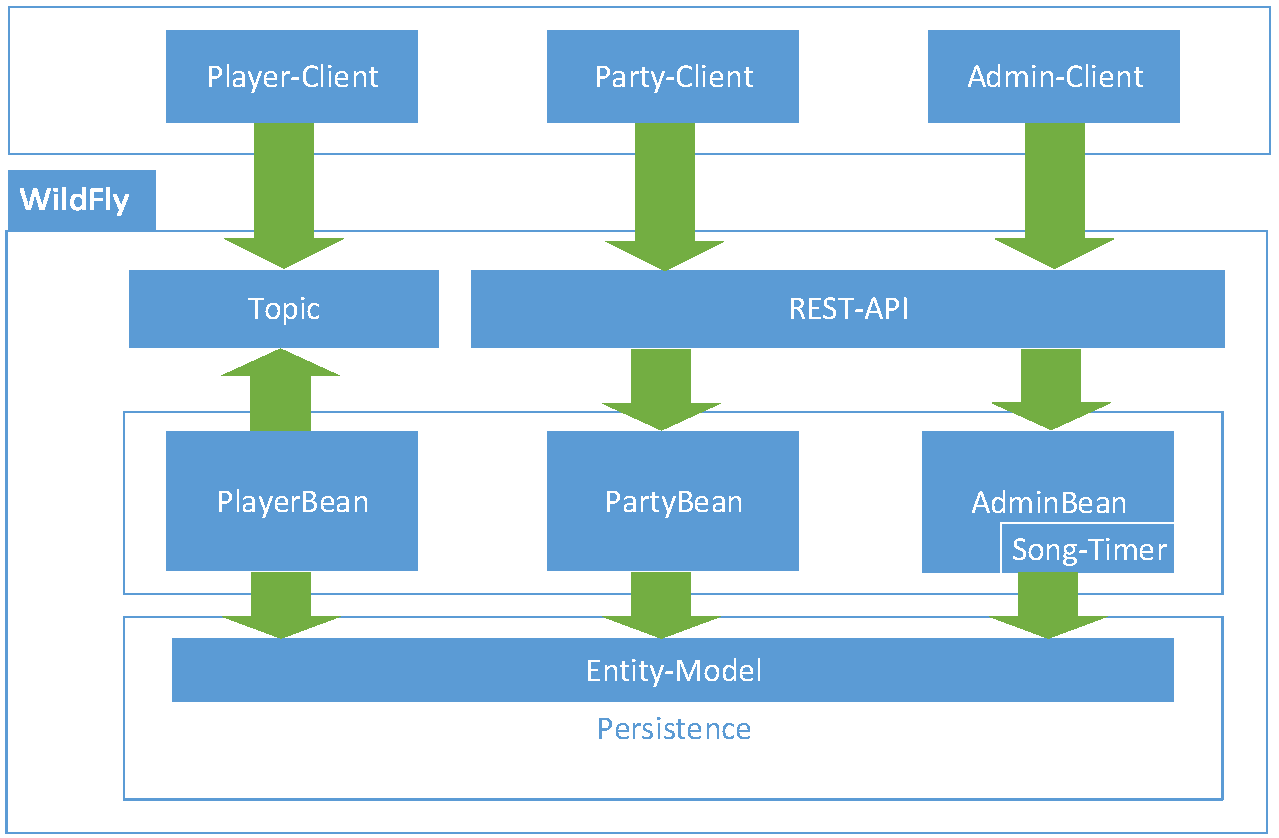
\includegraphics[width=1\linewidth]{Bilder/Komponentendiagramm_praesi}
	\caption{Komponentendiagramm der Systemübersicht }
	\label{fig:Komponentendiagramm}
\end{figure}

Die unterste Ebene mit dem Entity-Model beinhaltet die Persistenz-Logik. Mithilfe der JPA (Java Persistence API) und einer beliebigen Datenbank werden die Daten verwaltet.

Oberhalb dieser Ebene befinden sich die Beans, die allesamt das Entity-Model zur Persistierung der Daten benutzen. Es gibt eine PlayerBean, eine PartyBean und eine AdminBean.
Die PlayerBean sendet die zu spielenden Songs an ein Topic.
Die Aufgaben des AdminBeans umfassen das Verwalten der Songsammlung, das Starten einer Party, die damit verbundene Initialisierung der Playlist und die Auswahl der zu spielenden Songs. Beim Initialisieren der Playlist wird diese mithilfe des Song-Selection-Algorithmus (s. \ref{sec:SongSelect}) gefüllt. Die Anzahl der Einträge in der Playlist ist im AdminBean definiert. Weiter gehört zum Starten einer Party die Auswahl eines zu spielenden Songs. Beim Auswählen wird anhand der Song-Source ein Timer eingestellt, der nach der Länge (in Sekunden) des Songs ausgelöst wird. Dieser Timer initiiert die Persistierung des gespielten Songs für spätere Auswertungen und wählt den nächsten Song der Playlist aus. Bei jedem Auswählen eines zu spielenden Songs wird dieser aus der Playlist entfernt und über den Song-Selection-Algorithmus ersetzt.
Die PartyBean verwaltet die Votes und die DI-Werte der Party-People. Votes werden mit einem Song, einer positiven oder negativen Bewertung und der ID des Party-People persistiert. DI-Werte werden mit der Party-People-ID gespeichert.

Oberhalb der Bean-Ebene befindet sich das Topic, sowie die REST-API. Die Abhängigkeit der REST-API zu den Beans wird über Dependency-Injection aufgelöst. Ein Topic ist ein Messaging-Service, an den das PlayerBean den zu spielenden Song schickt, und der diesen an alle zu dem Zeitpunkt registrierten Player-Clients weiterleitet. Wir haben uns bewusst für ein Topic entschieden, da die Nachricht zum Abspielen eines Songs nur für einen kurzen Zeitraum relevant ist und nicht wie in einer Queue zwischengespeichert und zu einem späteren Zeitpunkt ausgeliefert werden soll.

Diese drei Schichten (Persistenz, Beans und REST-API) befinden sich allesamt im Applikationsserver WildFly, während die oberste Schicht\footnote{Diese Schicht wurde in diesem Projekt allerdings nicht mehr implementiert.} die verschiedenen Clients enthält. Der Player-Client empfängt die Song-Source vom Topic und spielt diese ab. Ein Party-Client kann Votes und DI-Werte an den Server senden. Der Admin-Client kann Songs und Partys verwalten.
\newpage

\subsection{Datenmodell}

In diesem Abschnitt wird das Datenmodell beschrieben. Dieses besteht aus Entitäten für die Objekte aus dem \nameref{sec:Domaenenmodell}, die persistiert werden sollen. Benutzer- und Rollendaten werden im Abschnitt \ref{sec:Benutzerrollen} beschrieben.

Abbildung \ref{fig:Datenmodell} zeigt die Entitäten sowie deren Beziehungen untereinander. Neben der Kardinalität ist in dem Diagramm auch das Cascading-Verhalten dokumentiert. Wir haben zwei unterschiedliche Arten verwendet:
\begin{description}
	\item[Refresh] Eine Entität kennt eine andere Entität. Änderungen oder Löschoperationen werden nicht an die verknüpfte Entität weitergeleitet (Abhängigkeit).
	\item[All] Eine Entität besitzt eine andere Entität. 
	Änderungen oder Löschoperationen werden an die 
	verknüpfte Entität weitergeleitet (Aggregation).
\end{description}

\vspace{8pt}
\begin{figure}[htb]
\centering
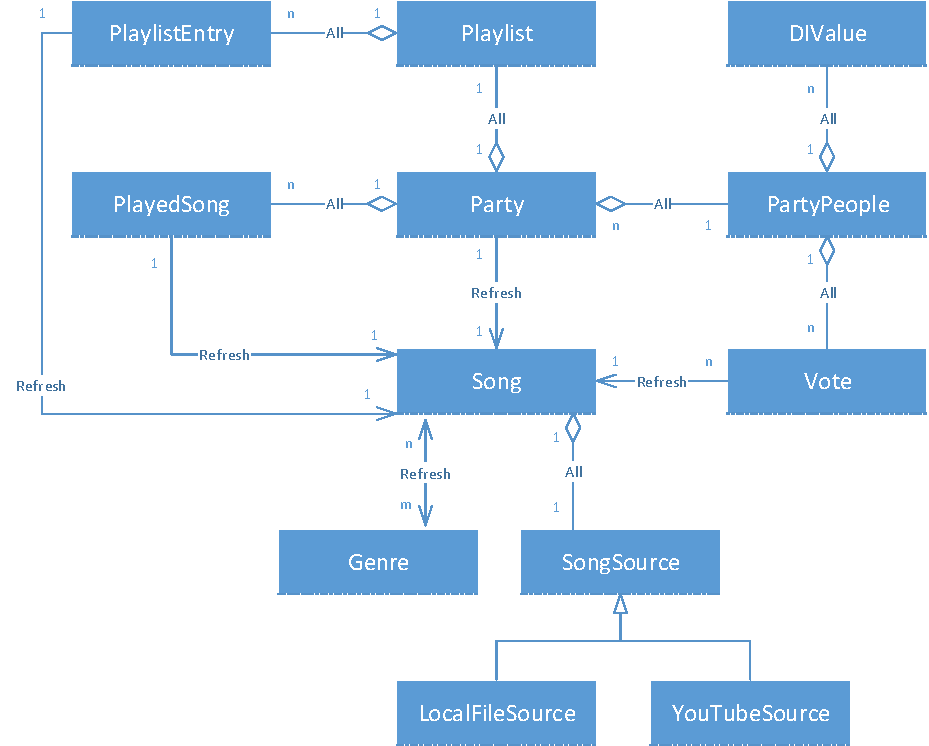
\includegraphics[width=1\linewidth]{Bilder/Datenmodell}
\caption{Datenmodell mit Beziehungen und Cascading zwischen Entitäten}
\label{fig:Datenmodell}
\end{figure}

Eine Anforderung an das Projekt ist es, möglichst alle Beziehungs- und Kardinalitätstypen sinnvoll anzuwenden. Aus diesem Grund werden im Folgenden relevante Beziehungen zwischen Entitäten und deren Kardinalitäten erläutert.

\begin{description}
	\item[One-To-One, Refresh] Eine Party kennt einen aktuellen Song. Da es immer nur eine laufende Party geben kann, ist ein Song auch maximal einer Party als aktueller Song zugeordnet. Der Cascading-Typ ist Refresh, weil beim Beenden einer Party der Song natürlich weiterhin in der Datenbank erhalten bleiben soll.
	\item[One-To-One, All] Ein Song hat eine SongSource. Eine SongSource enthält die Informationen zum Abspielen des Songs. Wird der Song geändert oder gelöscht, so soll sich dies direkt auf die SongSource auswirken.
	\item[Many-To-One, Refresh] Ein Vote kennt den Song, auf den sich die Bewertung bezieht. Ein Song kann von mehreren Votes bewertet worden sein. Änderungen oder Löschen eines Votes sollen keinen Einfluss auf die betroffenen Song-Daten haben.
	\item[One-To-Many, All] Eine Playlist besteht aus einer Liste von PlaylistEntry-Entitäten. Ein PlaylistEntry ist genau einer Playlist zugeordnet. Werden Änderungen an der Playlist vorgenommen, so sollen diese auch an die Einträge
	in der Liste weitergeleitet werden.
	\item[Many-To-Many, Refresh] Ein Song kann mehreren Genres zugeordnet werden. Zu einem Genre gehören beliebig viele Songs. Beim Löschen oder Ändern eines Songs soll das entsprechende Genre weiterhin bestehen bleiben und umgekehrt.
	\item[Inheritance] Eine SongSource kann mehrere Ausprägungen haben. Eine LocalFileSource identifiziert eine lokale Datei, während eine YouTubeSource ein Video auf YouTube identifiziert.
\end{description}



\subsection{Benutzerrollen}
\label{sec:Benutzerrollen}
Die Authentifizierung und Autorisierung von Benutzern erfolgt über das Sicherheitskonzept im WildFly. Dazu werden Benutzerrollen für die unterschiedlichen Anwender definiert. Der Zugriff auf Beans sowie die REST-Services wird über diese Rollen geregelt. 

\newpage
\subsubsection{Konzept}
Es gibt drei Benutzerrollen: Admin, Player und PartyPeople.
\begin{description}
	\item[Admin] Ein Administrator hat Zugriff auf das Admin-Bean und den Admin-Service, um Songs und Partys zu verwalten.
	\item[Player] Ein Player hat Zugriff auf das DJ-Topic, um Nachrichten zum Abspielen von Songs zu empfangen.
	\item[PartyPeople] PartyPeople haben als Gäste der Party Zugriff auf das Party-Bean und den Party-Service.
\end{description}

\subsubsection{Umsetzung}
Die Benutzer- und Rollendaten werden in der Datenbank gespeichert. Dazu wurden die zwei Entitäten Principal und Role angelegt. In der Datenbank wird zur Zuordnung zwischen Benutzern und Rollen eine zusätzliche Verknüpfungstabelle angelegt. Die Tabellen werden in Abbildung \ref{fig:BenutzerRollen} dargestellt.

\begin{figure}[tbh]
\centering
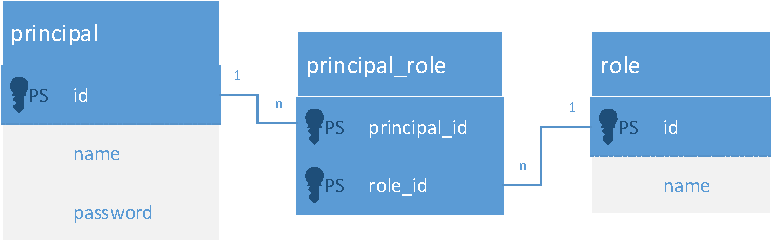
\includegraphics[width=0.8\linewidth]{Bilder/BenutzerRollen}
\caption{Tabellen für die Benutzerverwaltung}
\label{fig:BenutzerRollen}
\end{figure}

Im Standard verwendet WildFly die lokalen Benutzerdaten in den *.properties-Dateien. Um das Verhalten zu ändern, muss ein neues Login-Modul in der standalone.xml angelegt werden. In dieses Datenbank-Login-Modul wird die Datenquelle zusammen mit den SQL-Abfragen zur Bestimmung von Passwörtern und Rollen definiert. Aktuell werden die Passwörter im Klartext gespeichert. Für den produktiven Einsatz sollte hier auf ein aktuelles Hash-Verfahren wie SHA-2 umgestellt werden.

Um denselben Authentifizierungsmechanismus für Remote-Verbindungen und HTTP-Anfragen gegen den REST-Service zu nutzen, haben wir eine eigene Security-Realm sowie -Domain definiert. Zusätzlich war die Einstellung für Passwort-Stacking wichtig, da sonst entweder nur die Anmeldung über die REST-Schnittstelle oder über Remote möglich war. Die Zuordnung der Security-Domain zu den Beans und Services erfolgt über Annotationen an den entsprechenden Java-Klassen. 

\subsubsection{Probleme}
Die Authentifizierung war das größte Problem im gesamten Projekt und dem entsprechend auch mit dem höchsten Arbeitsaufwand verbunden. Selbst nach stundenlanger Recherche konnten einige Probleme aufgrund der eher mangelhaften Dokumentation und der wenig hilfreichen Fehlermeldungen nicht oder nur teilweise gelöst werden.

Besonders auffällig war, dass die einzelnen Features wie Remote-Authentifizierung einfach einzurichten waren. Sollte dieselbe Authentifizierung auch für REST-Service genutzt werden, mussten aufwendige und nicht dokumentierte Anpassungen an der WildFly-Konfiguration vorgenommen werden. Als gegen Ende des Projekts auch das Messaging authentifiziert werden sollte, konnten wir keine Lösung finden, mit der alle drei Schnittstellen korrekt arbeiteten. Aktuell funktioniert die Authentifizierung für Remote- und HTTP-Verbindungen. 


\subsection{Exemplarische Darstellung}
In diesem Abschnitt wird exemplarisch einen Funktionsaufruf der REST-API beschrieben. Da die verschiedenen über REST bereitgestellten Funktionen prinzipiell gleich implementiert sind, zeigt Abbildung \ref{fig:AufrufSequenz} den Ablauf der Funktion "`Party starten"'.

\begin{figure}[tbh]
\centering
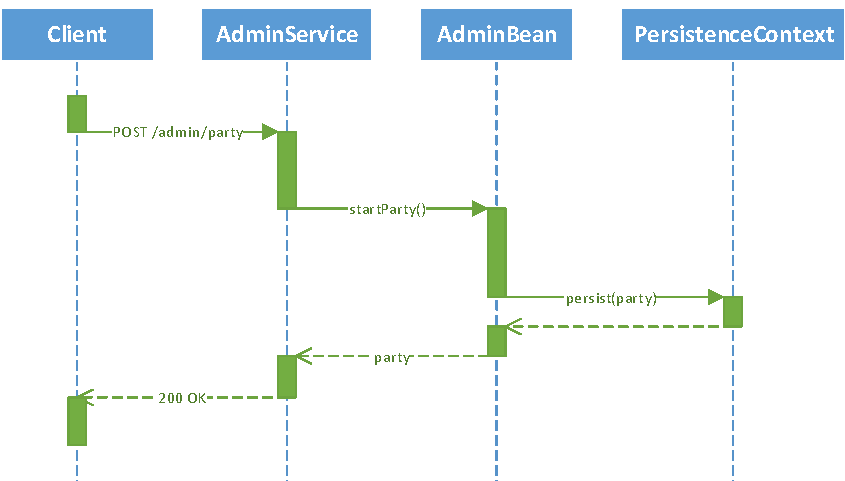
\includegraphics[width=1.0\linewidth]{Bilder/AufrufSequenz}
\caption{Sequenzdiagramm für den Start einer Party}
\label{fig:AufrufSequenz}
\end{figure}

Um eine Party zu starten, führt der Admin-Client einen HTTP-POST-Request unter der URI \textit{/admin/party} aus. Daraufhin wird im Admin-Service die startParty-Methode des Admin-Beans aufgerufen. Die Abhängigkeiten der Service- und der Bean-Klasse werden dabei über Dependency-Injection aufgelöst. Innerhalb des Admin-Beans wird eine neue Instanz der Entität Party erstellt und in der Datenbank persistiert. Abschließend gibt der Admin-Service den HTTP-Status-Code 204 zurück.

\subsection{Song-Selection-Algorithmus}
\label{sec:SongSelect}
Die Playlist wird über einen Algorithmus zur Auswahl von passenden Songs gefüllt. Dazu werden bekannte Kriterien der aktuellen Party wie Uhrzeit und durchschnittlicher Betrunkenheitsgrad berücksichtigt. Die Auswahl erfolgt auf Basis von bereits abgeschlossenen Partys, bei denen zu den gespielten Songs die notwendigen Daten gespeichert wurden.

\subsubsection{Definition}
Zunächst werden eine Reihe von Kennzahlen definiert, die der Algorithmus zur Auswahl des besten Songs benötigt.

\begin{description}
	\item[CDI] Current-Drunken-Index: Durchschnittlicher DI auf der aktuellen Party. Dieser wird als arithmetisches Mittel über die DI-Werte aller Party-People gebildet.
	\item[SDI] Song-Drunken-Index: Durchschnittlicher DI zu einem gespielten Song auf früheren Partys. Dieser Wert wurde beim Abspielen des Songs auf einer früheren Party in der Datenbank gespeichert.
	\item[$\Delta$DI] Definiert die maximale Abweichung des SDI vom CDI, unter der der Song als passend angesehen wird.
	\item[CTS] Current-Timestamp: Aktueller Zeitstempel der laufenden Party.
	\item[STS] Song-Timestamp: Zeitstempel zu einem gespielten Song auf früheren Partys. Dieser Wert wurde beim Abspielen des Songs auf einer früheren Party in der Datenbank gespeichert.
	\item[$\Delta$TS] Definiert die maximale Abweichung des SDS vom CTS, unter der der Song als passend angesehen wird.
\end{description}

\subsubsection{Algorithmus}
Der Algorithmus besteht aus zwei Schritten.
\begin{compactenum}
	
	\item Auswahl einer Menge an passenden Songs
	\item Auswahl des besten Songs aus den passenden Songs
\end{compactenum}

Zur Auswahl der passenden Songs werden gültige Bereiche von DI- und Timestamp-Werten definiert.
Diese Bereiche werden vergrößert, wenn keine passenden Songs gefunden wurden. Um eine Endlosschleife
zu vermeiden, wird diese Vergrößerung nur begrenzt oft durchgeführt. Konnten trotz mehrfacher 
Versuche keine Songs ermittelt werden, wird ein zufälliger Song aus der Songsammlung ausgewählt.
Wenn eine Menge von passenden Songs ermittelt werden konnte, wird der Song mit der besten
Bewertung durch die Party-People auf vergangenen Partys ausgewählt. Bei gleichem Vote-Count
entscheidet das Zufallsprinzip. 

Folgender Pseudocode skizziert den Algorithmus:
\begin{lstlisting}[language=C]
CDI = getCurrentAverageDI()
CTS = getCurrentTimestamp()
tries = 1
while (tries <= MAX_TRIES) {
	ΔDI = tries * DI_STEP
	ΔTS = tries * TS_STEP
	
	fittingSongs = SELECT * FROM PlayedSongs ps
                    WHERE ps.averageDI BETWEEN CDI - ΔDI AND CDI + ΔDI
                    AND    ps.timestamp BETWEEN CTS - ΔTS AND CTS + ΔTS
				   	 
	Remove from fittingSongs: 
	  Already played songs on this party
	  Current song on this party
	  Songs in current playlist
		
	if (fittingSongs is not empty) {
	  bestSong = choose song with max vote count from fittingSongs
	  return bestSong
	}
	
	tries = tries + 1
}
return randomSong()
\end{lstlisting}